% !TeX root = e4-tp2-ej2
\documentclass[e4-tp2-main.tex]{subfiles}

\begin{document}

\section{Convertidor boost para l\'ampara LED de potencia}

\subsection{Efectos de temperatura en los LEDs}

\begin{wrapfigure}[15]{L}{0.50\textwidth}
    \centering
    \begin{subfigure}[t]{0.24\textwidth}
    	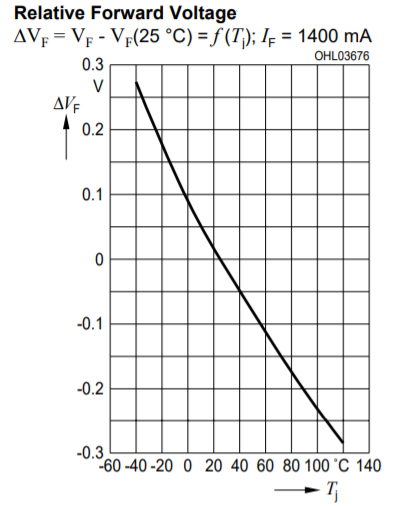
\includegraphics[width=\textwidth]{images/ej2/Cambio_Vf_LED.png}
    	\caption{Cambios en $V_f$}
    \end{subfigure}
    \begin{subfigure}[t]{0.24\textwidth}
    	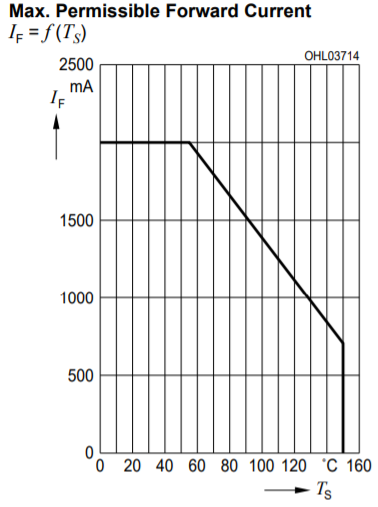
\includegraphics[width=\textwidth]{images/ej2/Cambio_If_LED.png}
    	\caption{Cambios en $I_{f_{MAX}}$}
    \end{subfigure}
    \caption{Efectos de la temperatura en los LEDs}
    \label{fig:Efec_Leds}
\end{wrapfigure}

Se utilizaron los LEDs OSRAM LUW-W5AP, los cuales a medida que aumenta su temperatura se producen variaciones de la tensión de forward ($V_f$) y la máxima corriente de forward soportada ($I_{f_{MAX}}$). Donde ante un aumento de la temperatura tenemos un aumento de $V_f$ y una disminución de $I_{f_{MAX}}$.\\

Como puede observarse de los gráficos obtenidos del datasheet en la figura \ref{fig:Efec_Leds} se puede despreciar los cambios producidos en $V_f$ debido a que los cambios de corriente son mucho más apreciables y los cambios en $V_f$ no afectan tanto el comportamiento del circuito.\\

\subsection{Cambio en el brillo}

Dado que los leds son ideales y cada uno tiene la misma caída de tensión, tenemos que en cada diodo caen $V_f=3,4V$. Dado que se utiliza un convertidor BOOST, tenemos $V_o=V_g\cdot\frac{1}{1-D}$ donde se fija $V_o$ y como la corriente de salida va a haberse dominada por la resistencia $R_2$, por $I_o=\frac{V_{out}-4\cdot V_f}{R_2}$. Podemos observar que los cambios en $I_o$ son inversamente proporcionales para $R_2$.\\
Para el caso del brillo al $100\%$ necesitamos $I_o=2A$ y para el $100\%$ necesitamos $I_o=0,76 A$, por lo tanto $R_{2(50\%)}=\frac{2}{0,76}\cdot R_{2(100\%)}$.\\

\subsection{Tiempo de establecimiento al 5\%}

\end{document}

